\documentclass{scrartcl}

\usepackage{graphicx}


\usepackage[font=small,skip=4pt]{caption}

\title{3D Geometric Data Structure, a Survey\vspace{-4ex}}

\setlength\parindent{0pt}

\begin{document}
\maketitle

\textbf{Abstract}
\begin{abstract}
	We compare DSC with other index-based data structure (e.g. VTK) and cell complexes (generalized half edge, e.g. CGAL). DSC is 100 times faster than cell-complexes methods. In index-based category, DSC belong to good performance but high memory group. 
	
	Performance of DSC can still be increased: four times with additional three functions or ten times if full adjacency information are stored. This analysis is mainly based on theoretical, practice may differ.
\end{abstract}

%%%%%%%%%% Section catergories
%\noindent
\textbf{Tetrahedral representation categories}

\begin{itemize}
	\setlength\itemsep{0em}
	\item Index-based data structures: No adjacency (VTK \cite{vtk}); with adjacent information \cite{Schroeder1988, Shephard1991}, DSC \cite{Misztal2012}; and reduced data structure with adjacent information \cite{Beall1997, Garimella2002} 
	\item Cells complex OpenVolume Mesh\cite{Kremer2013} and (CGAL) \cite{CGAL} 
\end{itemize}

%%%%%%%%% Section compare index
%\noindent
\textbf{Comparison of index-based data structure}

Adjacency references and comparison of time-use in DSC is shown in Fig. \ref{fig:dsc:stat}.

\begin{figure*}[!htb]
	\centering
	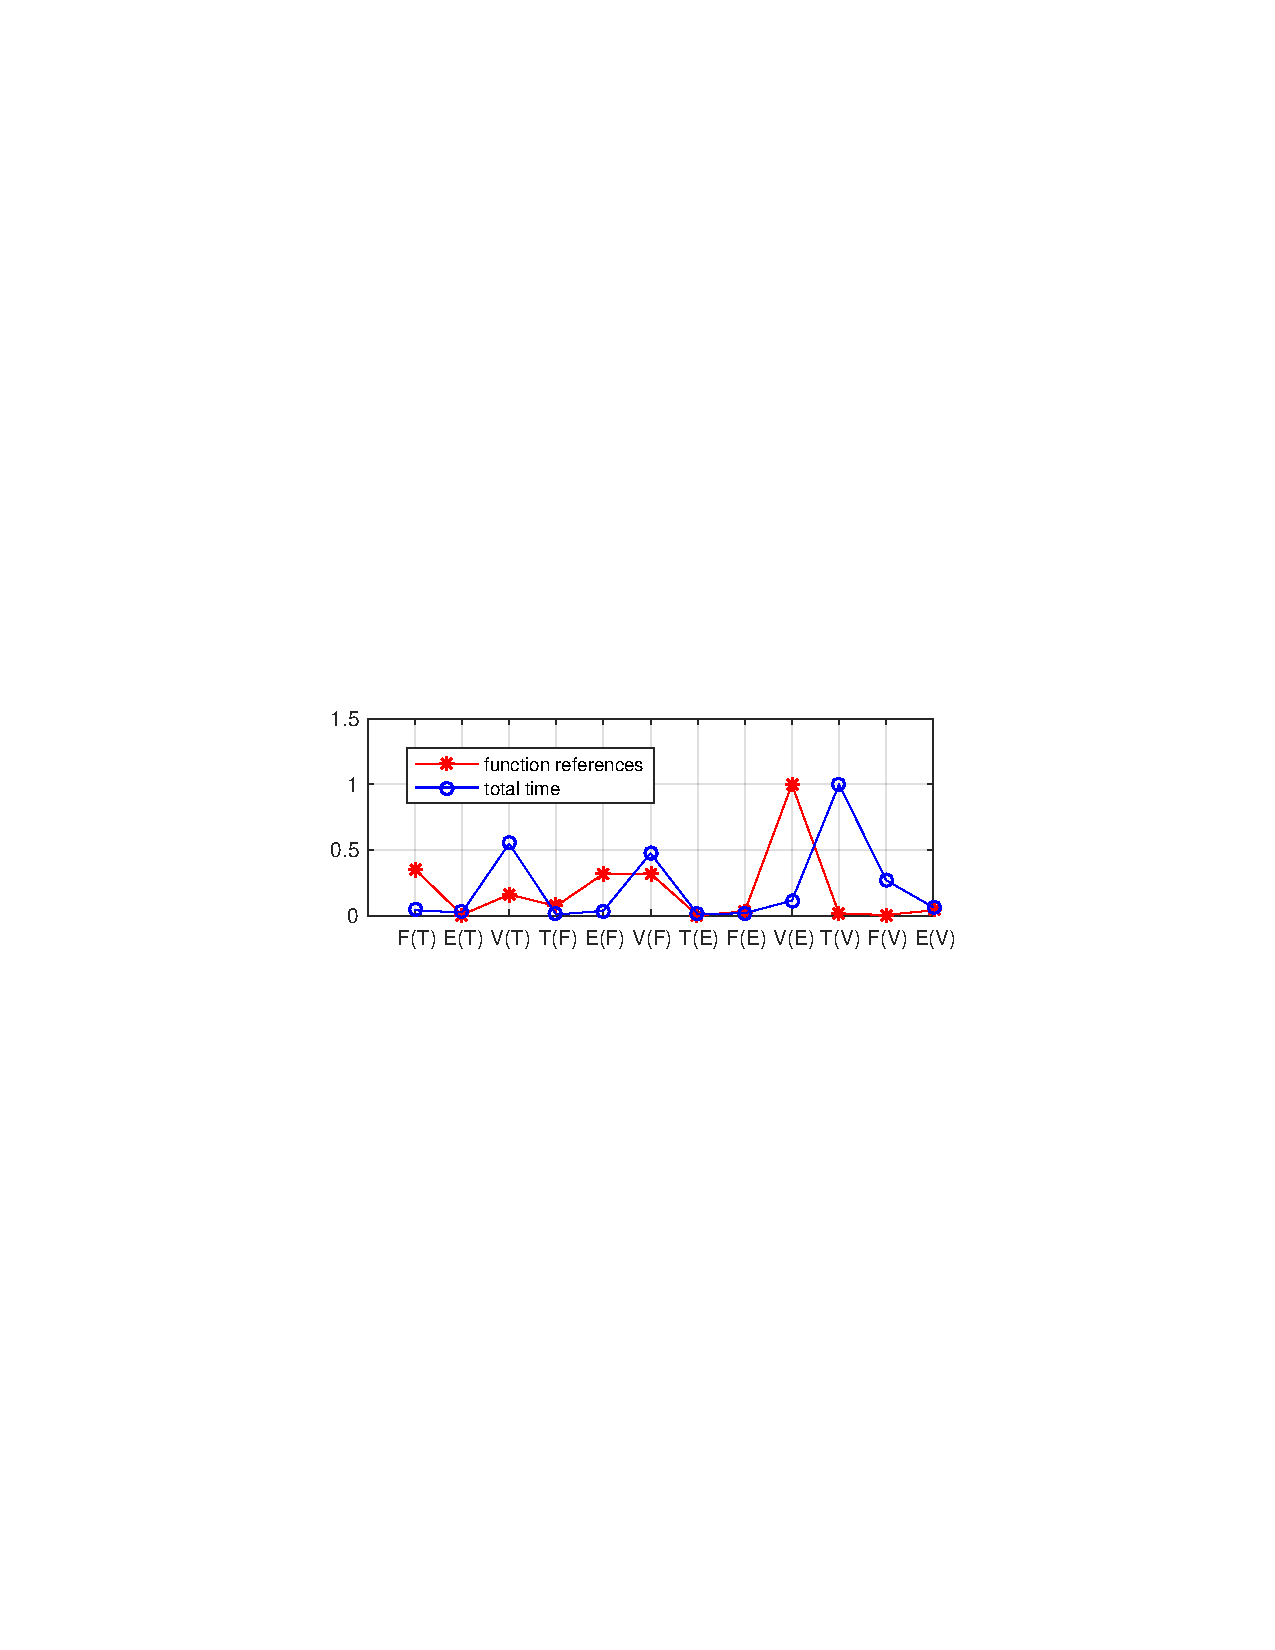
\includegraphics[height=11em]{../ref_time}
	\caption{Comparison of adjacency references and total time used of each function in DSC. F(T) means get face on tet, V(E) means get vertices on edge, etc...}
	\label{fig:dsc:stat}
\end{figure*}

Comparison of DSC and other index-based methods in term of performance and memory\footnote{We follow a theoretical comparison from \cite{Garimella2002}: A statistics of adjacencies references is measured by real usage of DSC (red line in Fig. \ref{fig:dsc:stat}), and the computation costs of functions to get adjacent information are estimated from the algorithms.}
is shown in Fig. \ref{fig:index:compare}. We compare different way to store adjacency information, including DSC, nine other index-based mesh \cite{Garimella2002}, DSC with additional storage of 3 functions (tet-vertex, vertex-tet and vertex-face), and full adjacencies (Fig. \ref{fig:methods}).


\begin{figure*}[!htb]
	\centering
	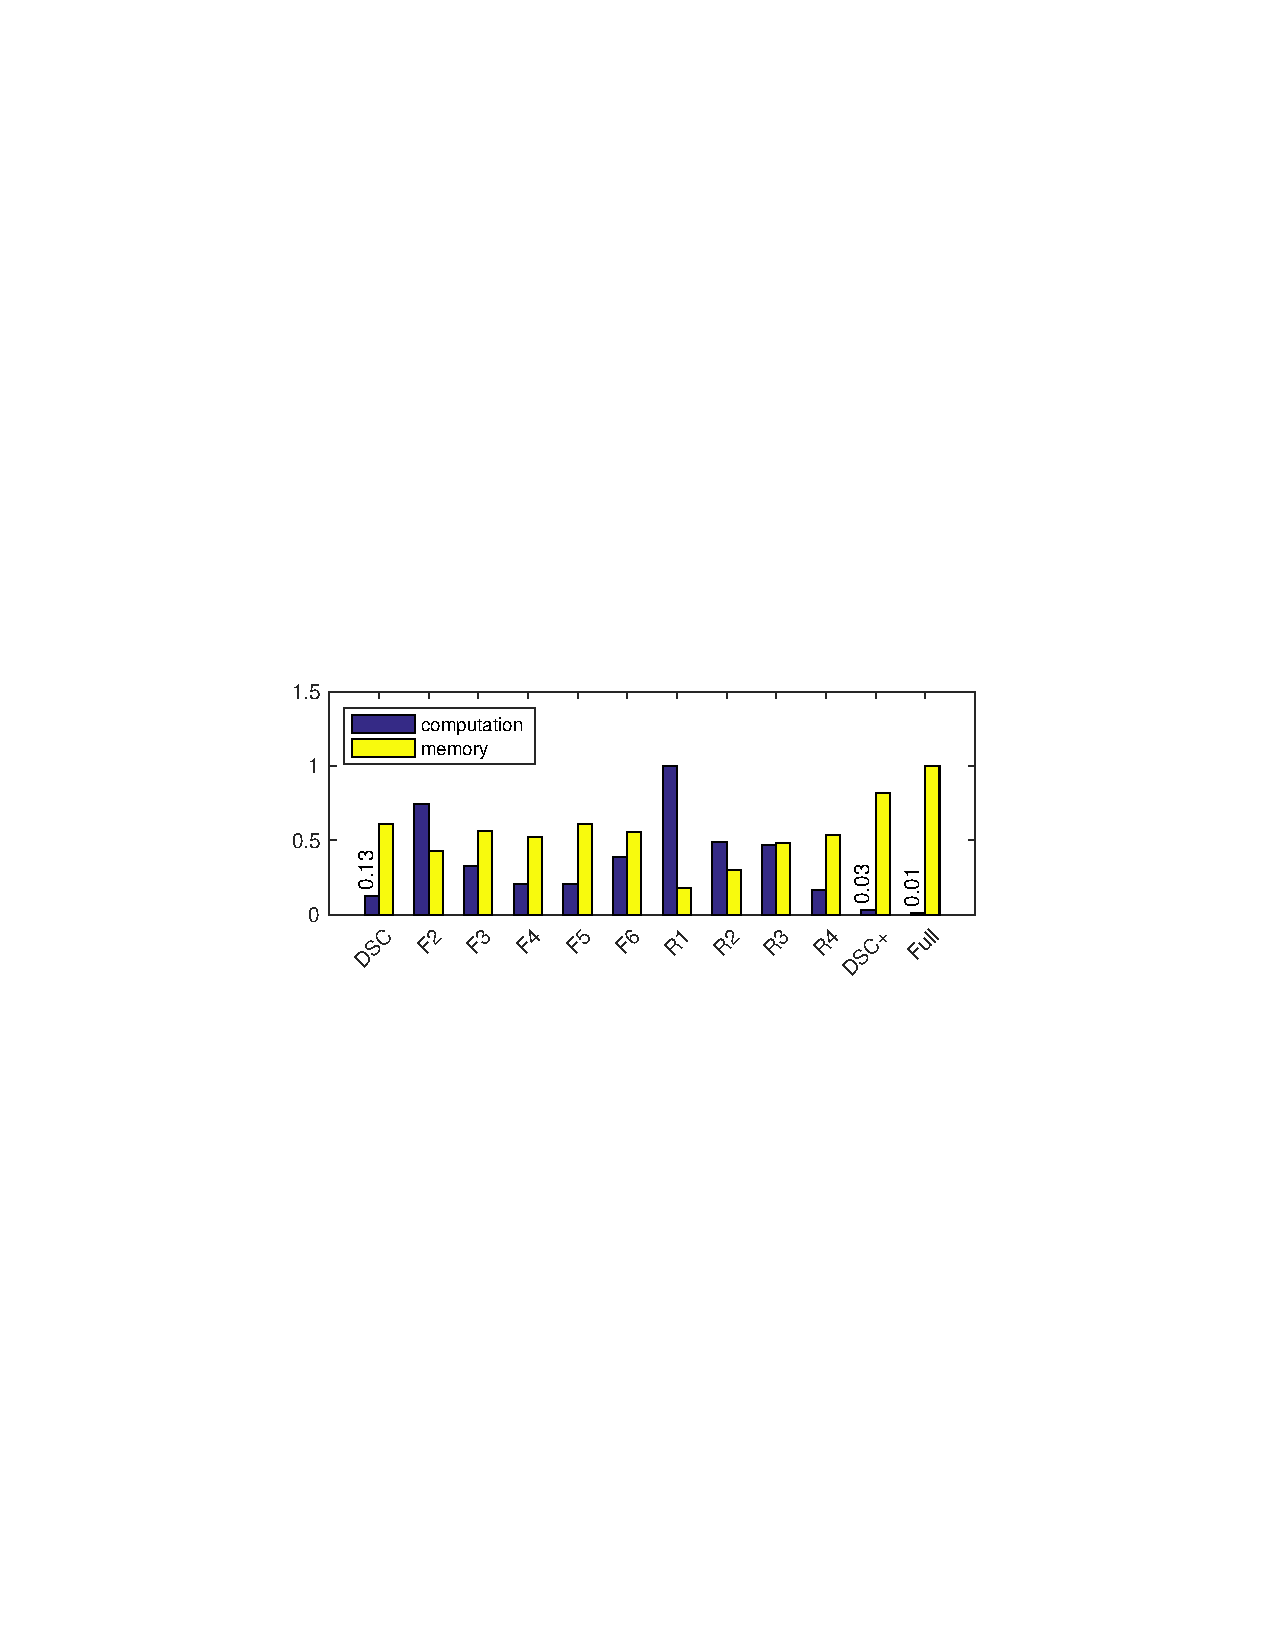
\includegraphics[height=12em]{../compute_mem}
	\caption{Memory and computation}
	\label{fig:index:compare}
\end{figure*}



Comparison between DSC and CGAL (linear cells complex \cite{CGAL}) is shown in Fig. \ref{fig:compare:cellcomplex}


\begin{figure*}[!htb]
	\centering
	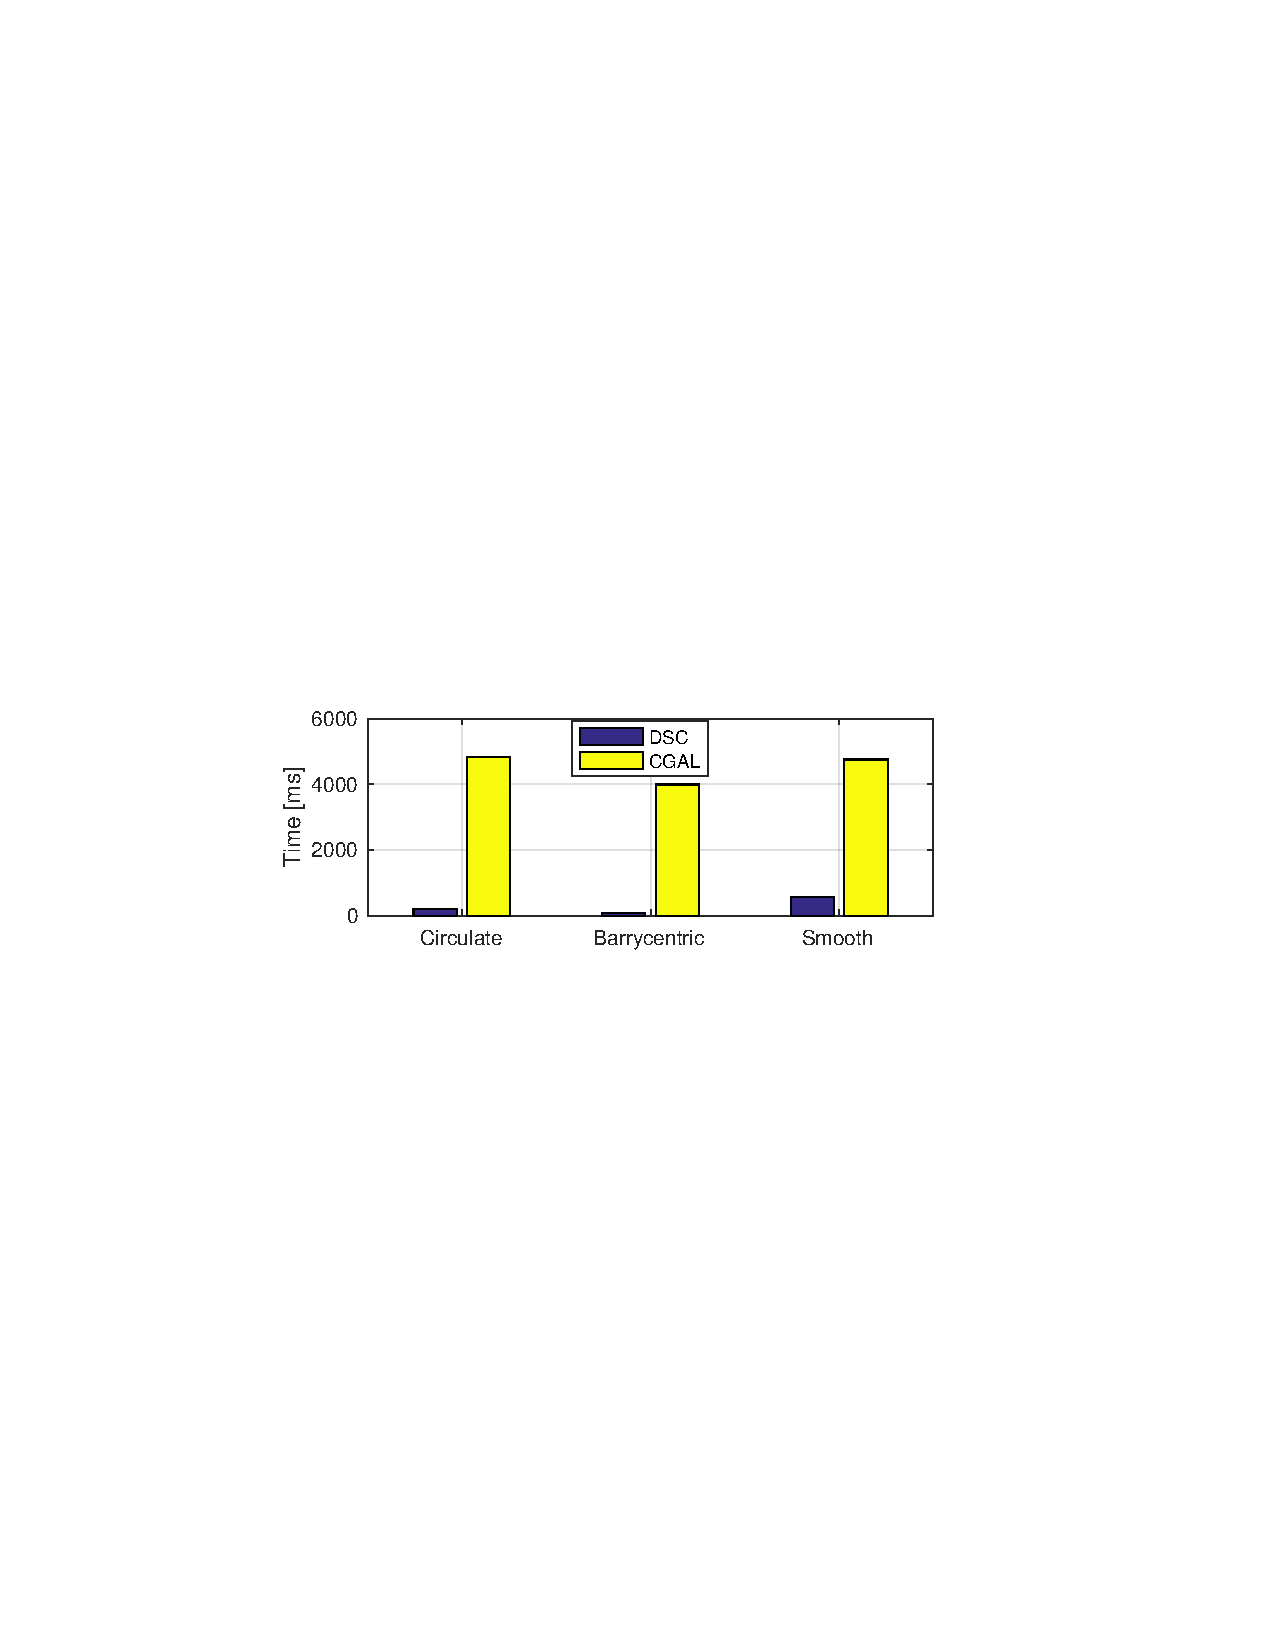
\includegraphics[height=11em]{../dsc_cgal}
	\caption{Comparison of DSC and CGAL}
	\label{fig:compare:cellcomplex}
\end{figure*}


\begin{figure*}
	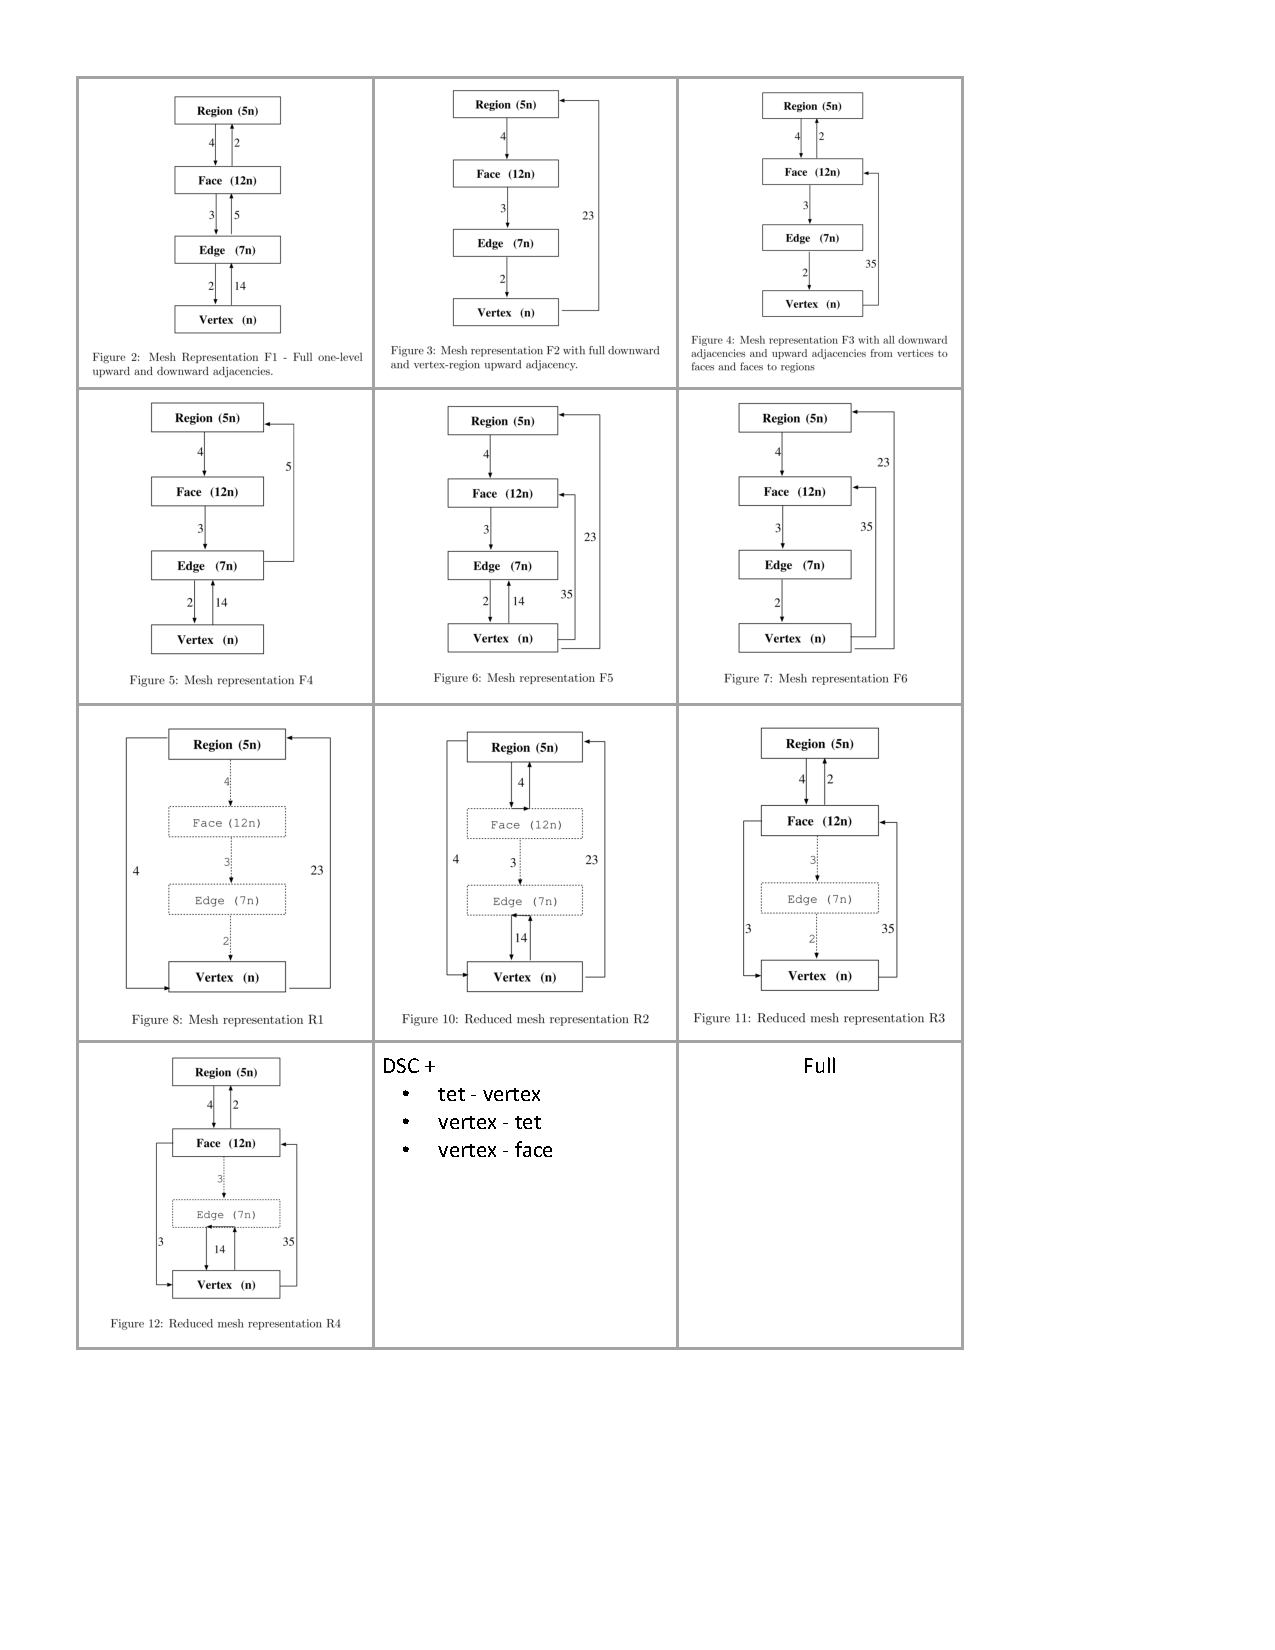
\includegraphics[scale=0.98]{../DSC}
	\caption{Methods for comparison of index-based data structure \cite{Garimella2002}}
	\label{fig:methods}
\end{figure*}

\bibliographystyle{plain}
\bibliography{citation.bib}

\end{document}

